\section{Benchmarks}

The following benchmarks were performed individually for each of the previously mentioned Kernel modifications on an Arch Linux Virtual Machine. To empirically measure the throughput and turnaround time of various workloads, Prime95 was used to stress test the various Kernel builds. In addition, a custom built C++ program was used to run a synthetic workload on 16 concurrent child processes, calculated the average time required to finish each process.

The benchmarks used were as follows:
\begin{itemize}
	\item Prime 95 Benchmark, sampled when running 25 iterations of 2048K FFT on 1, 2 and 4 cores.
	\item SyntheticProcess, our custom C++ synthetic load program, running 16 child processes each running a synthetic load and then averaging the completion time of all children (with a 1 sec delay between iterations to ensure the children were dequeued completely).
	\item A composite test where Prime 95 and SyntheticProcess are run in parallel to evaluate CFS's ability to share between entirely separate pid parents.
\end{itemize}

\noindent The Kernels used in our benchmarks were as follows:
\begin{description}
	\item[STOCK] A stock build of Linux 4.2.6
	\item[Test1] A modified version of the stock Kernel, implementing the pick\_next\_task psudocode changes detailed above.
	\item[Test2] A stock build of Linux 4.2.6 with the following Kernel parameters configured using \texttt{sysctl}:
	
		sched\_rt\_period\_us = 10,
		
		sched\_rt\_runtime\_us = 10,
		
		sched\_rr\_timeslice\_ms = 1,
		
		sched\_cfs\_bandwidth\_slice\_us = 1
	\item[Test3] A modified version of the stock Kernel, implementing the CFS Bandwidth and Quota changes detailed above. Specifically, RUNTIME\_INF was set to 10\% of the CFS bandwidth period (previously it was unrestricted), refill\_cfs\_bandwidth\_runtime() was short circuited to disable refilling alloted bandwidth, and the sched.h preprocessor constant MAX\_SHARES was changed from $2^{18}$ to $2^9$.
\end{description}

\vspace{1pc}
\noindent\textbf{Benchmark Results}
\vspace{1pc}

As can be seen from the benchmark results, Prime 95 performed nearly identical on all variants of the Kernel, with very little variance. Likewise, our Synthetic load program also saw nearly identical results for all Kernel variants, with only a 0.001 second variance between each test.

Interestingly, Prime 95 saw a significant amount of variance during the composite test during it's 2 core run on all Kernels. This may be a result of CFS struggling to decide which Kernel threads to map with process threads, resulting in frequent process migrations between cores. This hypothesis can be backed up by the fact that the results were very consistent when Prime 95 is run on all 4 cores, when all Kernel threads must be utilized all the time. Additionally, the Synthetic load also saw a considerable degree of variance between tests (range of 0.06 sec) during the same composite test with Prime 95, meaning that CFS's scheduling decisions effected both processes.

\begin{figure}[hb]
	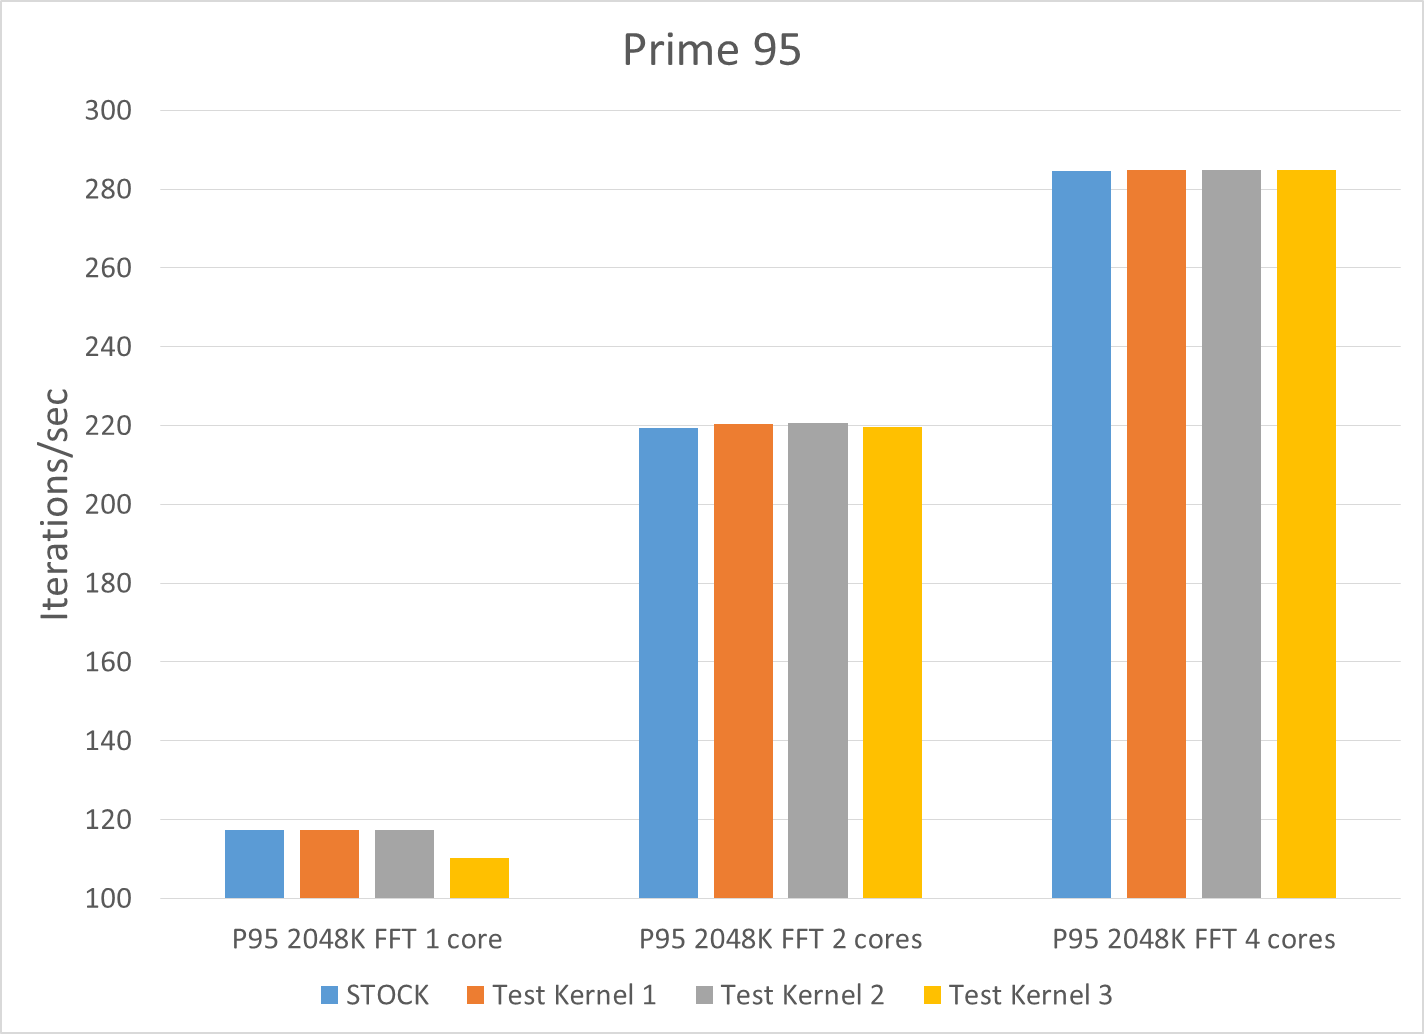
\includegraphics[width=1.0\columnwidth]{images/P95}
	\caption{Prime 95 Benchmark sampled at 2048K FFT on 1, 2, and 4 cores}
\end{figure}

\begin{figure}[hb]
	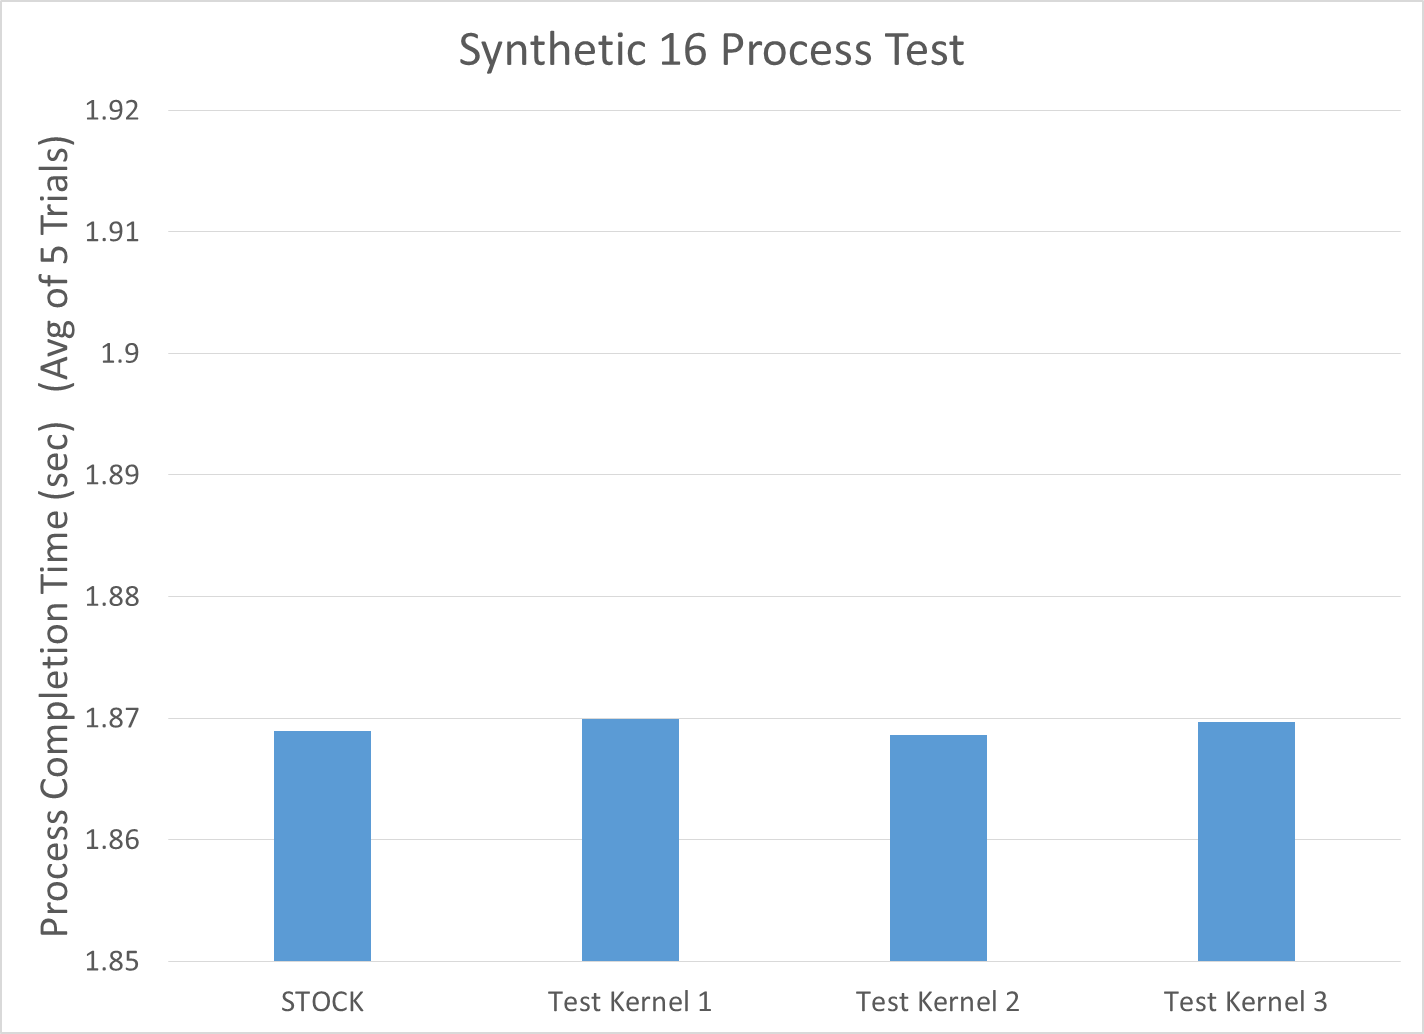
\includegraphics[width=1.0\columnwidth]{images/Synthetic}
	\caption{Synthetic load, completion time of each forked process, averaged over 5 trials of batches of 16 concurrent forks.}
\end{figure}

\begin{figure}[hb]
	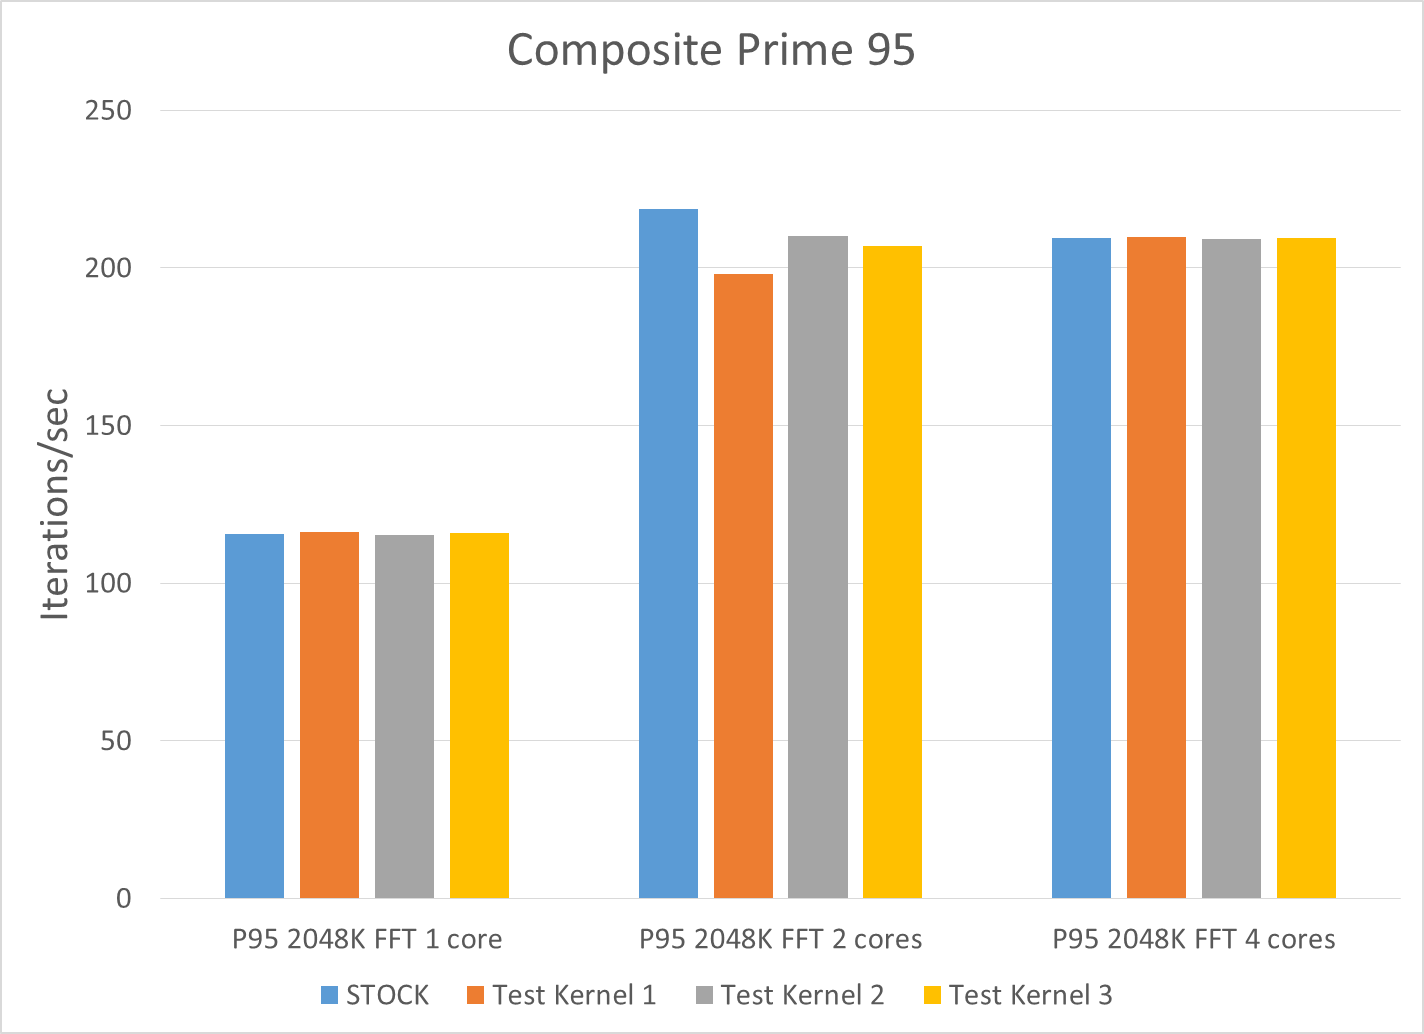
\includegraphics[width=1.0\columnwidth]{images/CompositeP95}
	\caption{Composite test running both Prime 95 and Synthetic load at the same time. A high amount of variance can be observed while Prime 95 was running on only 2 cores.}
\end{figure}

\begin{figure}[hb]
	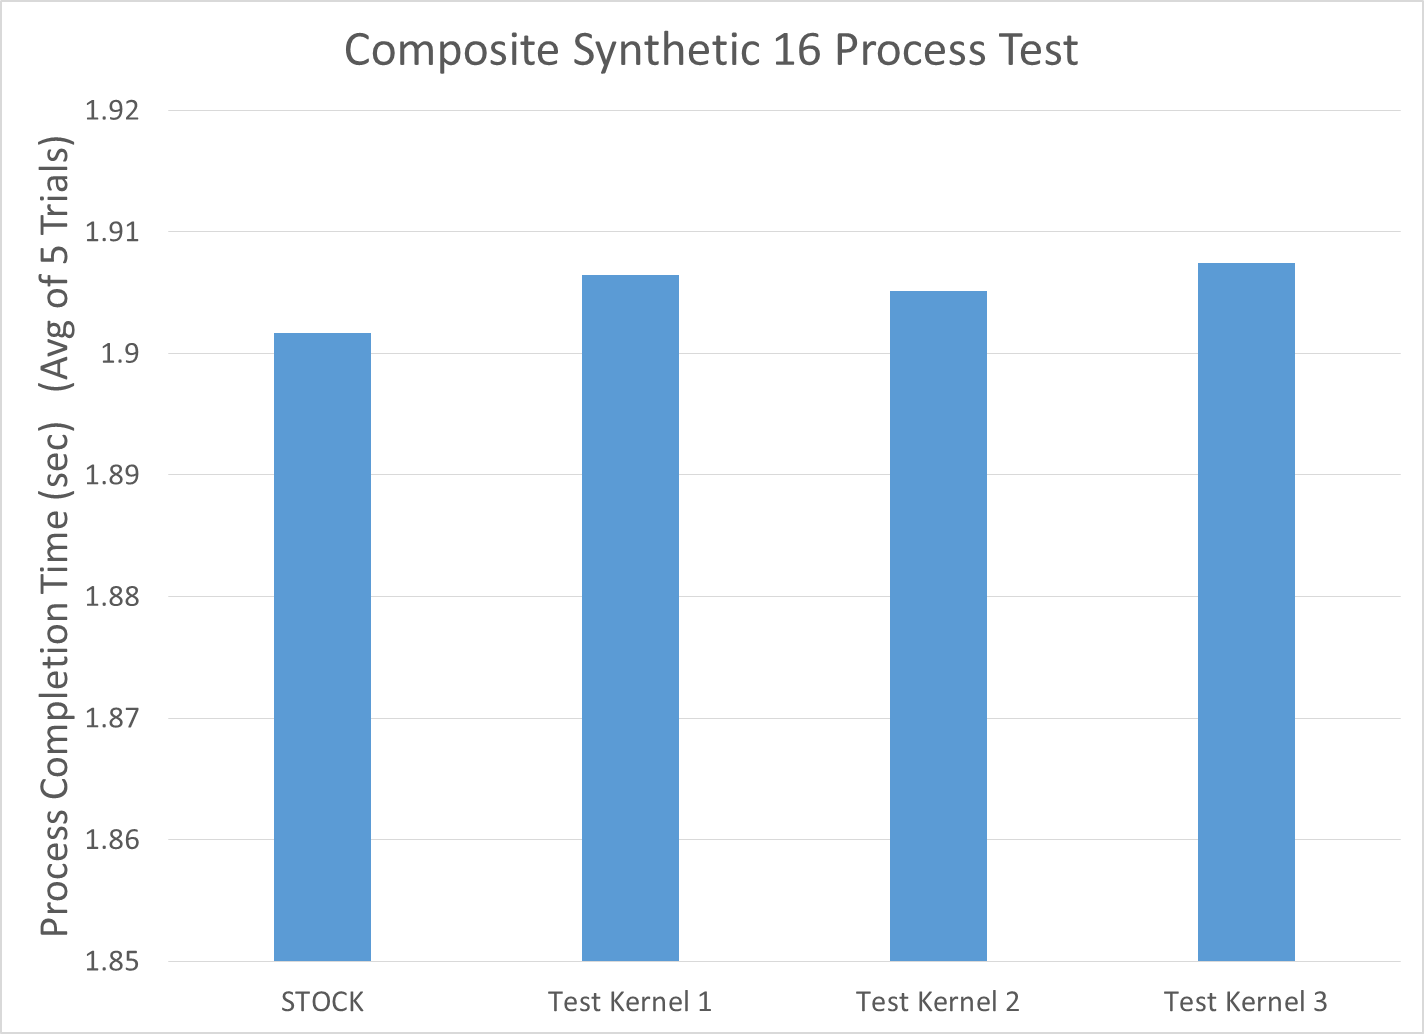
\includegraphics[width=1.0\columnwidth]{images/CompositeSynthetic}
	\caption{The same composite test, running both Prime 95 and Synthetic load at the same time. Each sample represents the average of the last 5 iterations of Synthetic load while Prime 95 was completing it's 2048K FFT run.}
\end{figure}

\vspace{20pc}
